\textbf{Целью первой лабораторной работы} является освоение возможностей программы Microsoft Project для планирования проекта по разработке программного обеспечения.

\section*{Задание для тренировки}

При создании плана пробного проекта использовались параметры рабочей среды Microsoft Project, заданные по умолчанию. Для типа задач по умолчанию используется фиксированный объем ресурсов. Настройки показаны на рисунке \ref{img:task0-settings}.

\begin{figure}[H]
	\begin{center}
		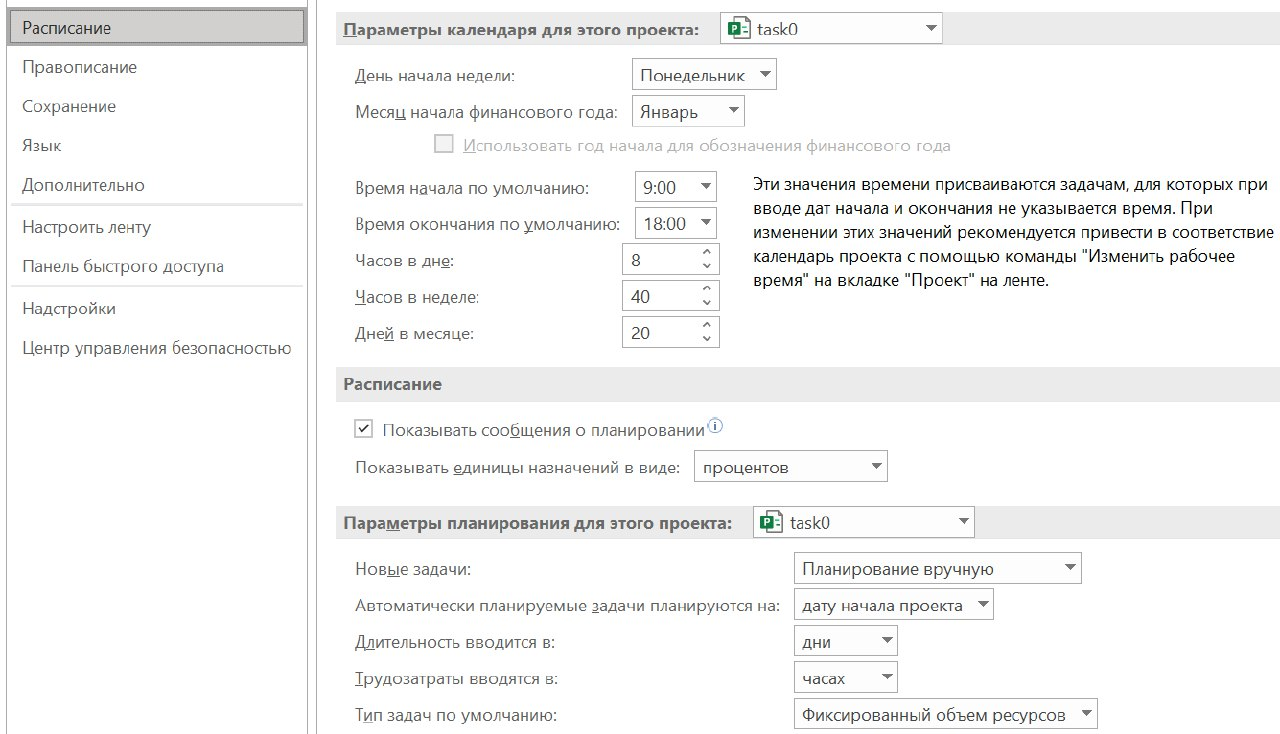
\includegraphics[scale=0.42]{inc/img/task0-settings.jpg}
	\end{center}
	\captionsetup{justification=centering}
	\caption{Параметры рабочей среды Microsoft Project}
	\label{img:task0-settings}
\end{figure}

Установка даты начала проекта в первый рабочий день марта текущего года представлена на рисунке \ref{img:task0-start-date}.

\begin{figure}[H]
	\begin{center}
		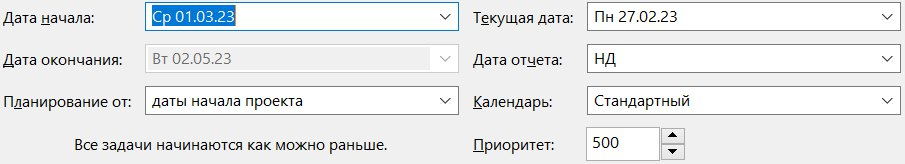
\includegraphics[scale=0.5]{inc/img/task0-start-date.jpg}
	\end{center}
	\captionsetup{justification=centering}
	\caption{Дата начала проекта}
	\label{img:task0-start-date}
\end{figure}

Было осуществлено планирование проекта со временными характеристиками, приведенными в таблице \ref{tab:tasks}.

\begin{table}[h]
    \caption{Временные характеристики проекта}
    \begin{center}
        \begin{tabular}{|l|l|}
        		\hline
            \multicolumn{1}{|c}{\textbf{Название работы}} & 
            \multicolumn{1}{|c|}{\textbf{Длительность (дни)}} \\ \hline
            Работа A & 12 \\ \hline
            Работа B & 6 \\ \hline
            Работа C & 10 \\ \hline
            Работа D & 7 \\ \hline
            Работа E & 9 \\ \hline
            Работа F & 8 \\ \hline
            Работа G & 10 \\ \hline
            Работа H & 10 \\ \hline
            Работа I & 6 \\ \hline
            Работа J & 5 \\ \hline
        \end{tabular}
    \end{center}
    \label{tab:tasks}
\end{table}
\newpage
При этом были учтены следующие связи между задачами:

\begin{enumerate}
	\item D --- исходная работа проекта.
	\item Работы С, E и F начинаются сразу по окончании работы D.
	\item Работы A и J следуют за C, а работа G --- за F.
	\item Работа I следует за A, а работа B --- за G.
	\item Работа H начинается после завершения E, но не может начаться, пока не
завершены I и B.
\end{enumerate}

Построенная диаграмма Ганта показана на рисунке \ref{img:task0}. Из полученного результата видно, что длительность проекта составила 45 дней, датой завершения работ является вторник 02.05.2023.

\begin{figure}[H]
	\begin{center}
		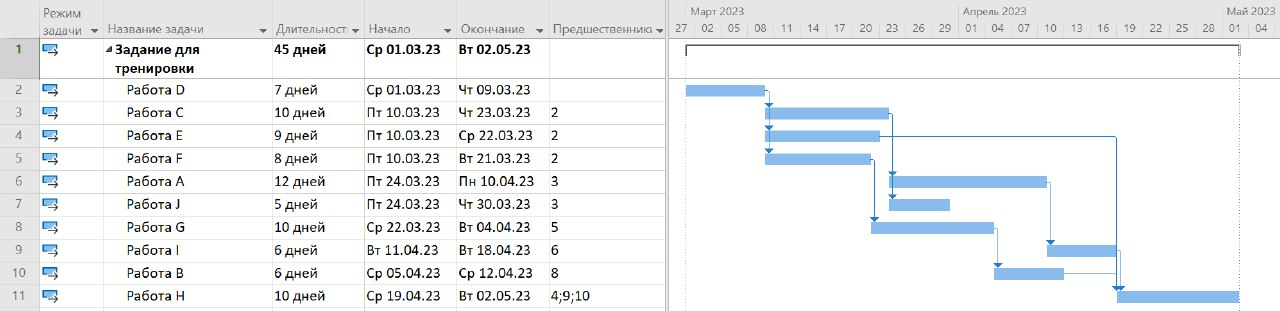
\includegraphics[scale=0.5]{inc/img/task0.jpg}
	\end{center}
	\captionsetup{justification=centering}
	\caption{Построенная диаграмма Ганта}
	\label{img:task0}
\end{figure}

\section*{Содержание проекта}

Команда разработчиков из 16 человек занимается созданием карты города на основе собственного модуля отображения. Проект должен быть завершен в течение шести месяцев. Бюджет проекта: 50 000 рублей.

\section*{Задание 1}

Установка даты начала проекта в первый рабочий день марта текущего года представлена на рисунке \ref{img:task0-start-date}.

\begin{figure}[H]
	\begin{center}
		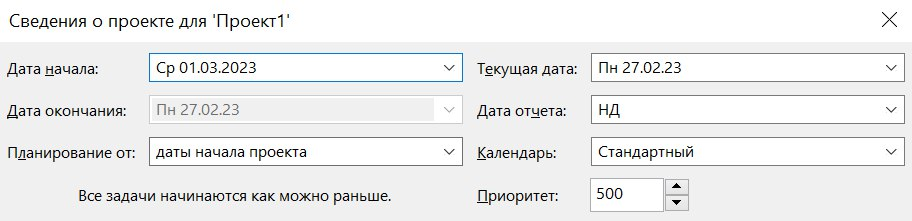
\includegraphics[scale=0.42]{inc/img/task1-start-date.jpg}
	\end{center}
	\captionsetup{justification=centering}
	\caption{Дата начала проекта}
	\label{img:task1-start-date}
\end{figure}

При создании плана были установлены следующие значения параметров: длительность работы --- в неделях, объем работ --- в часах, тип работ --- с фиксированными трудозатратами, количество рабочих часов --- восемь, количество рабочих часов в неделю --- 40, начало рабочей недели --- понедельник, начало финансового года --- январь, продолжительность рабочего дня --- 9:00-18:00. Настройки приведены на рисунке \ref{img:task1-settings}.

\begin{figure}[H]
	\begin{center}
		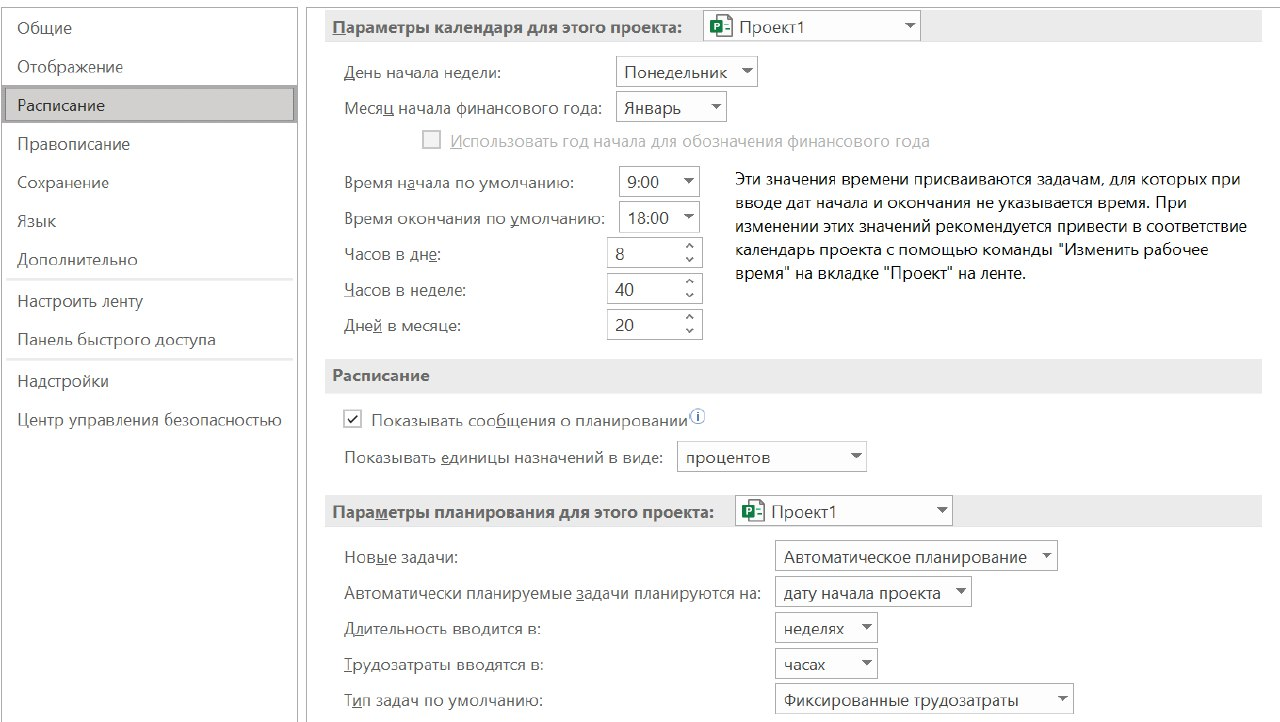
\includegraphics[scale=0.4]{inc/img/task1-settings.jpg}
	\end{center}
	\captionsetup{justification=centering}
	\caption{Параметры рабочей среды Microsoft Project}
	\label{img:task1-settings}
\end{figure}

На рисунке \ref{img:task1-calendar} показана установка стандартного календаря рабочего времени и создание праздничных дней на ближайшие семь календарных месяцев от даты начала проекта.

\begin{figure}[H]
	\begin{center}
		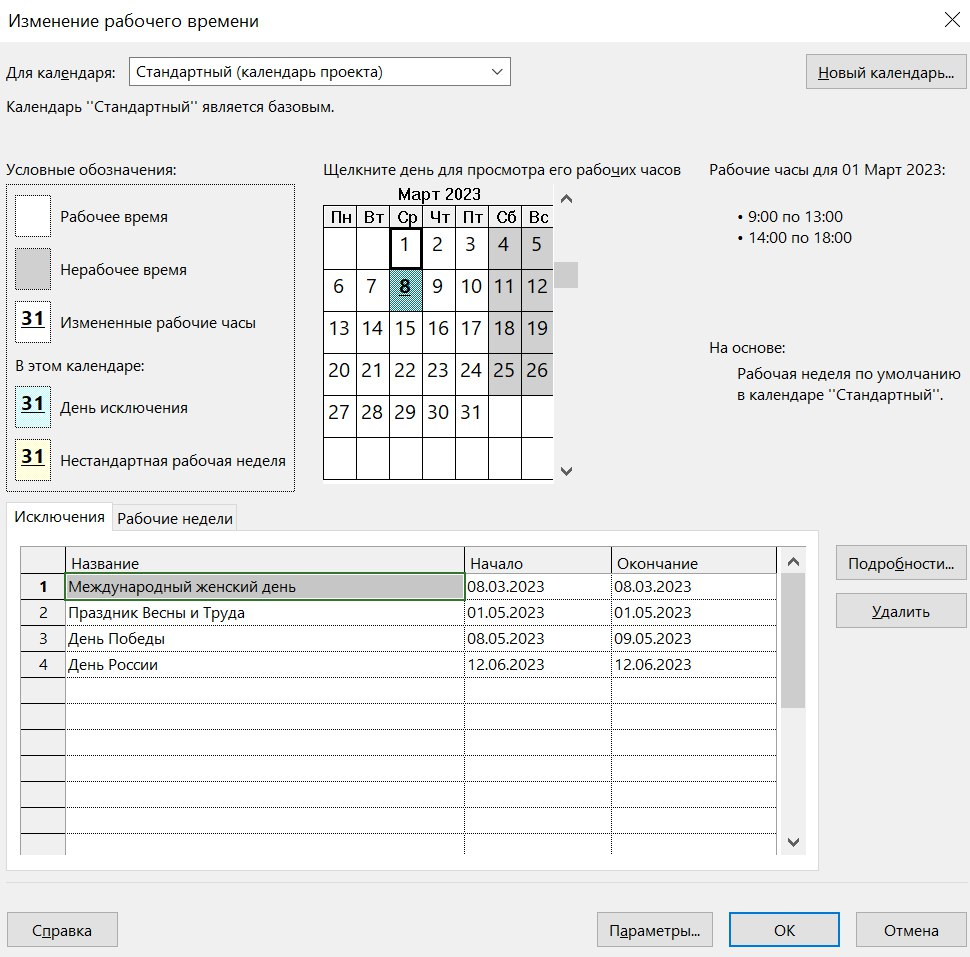
\includegraphics[scale=0.4]{inc/img/task1-calendar.jpg}
	\end{center}
	\captionsetup{justification=centering}
	\caption{Изменение рабочего времени}
	\label{img:task1-calendar}
\end{figure}

После вывода на экран суммарной задачи проекта вкладка <<Заметки>> была заполнена информацией о содержании проекта, как представлено на рисунке \ref{img:task1-description}.

\begin{figure}[H]
	\begin{center}
		
\includegraphics[scale=0.4]{inc/img/task1-description.jpg}
	\end{center}
	\captionsetup{justification=centering}
	\caption{Изменение рабочего времени}
	\label{img:task1-description}
\end{figure}

\section*{Задание 2}

Был создан список задач проекта, приведенный на рисунке \ref{img:task2}.

\begin{figure}[H]
	\begin{center}
		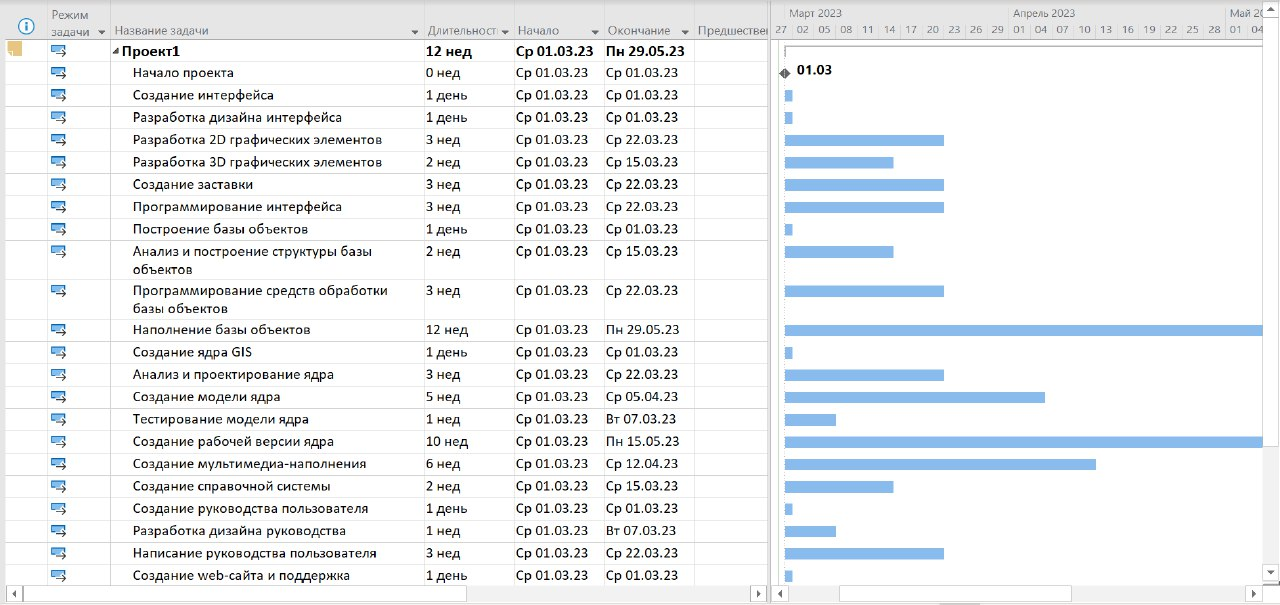
\includegraphics[scale=0.5]{inc/img/task2.jpg}
	\end{center}
	\captionsetup{justification=centering}
	\caption{Список задач проекта}
	\label{img:task2}
\end{figure}

\section*{Задание 3}

Структурированный список задач проекта показан на рисунке \ref{img:task3}.

\begin{figure}[H]
	\begin{center}
		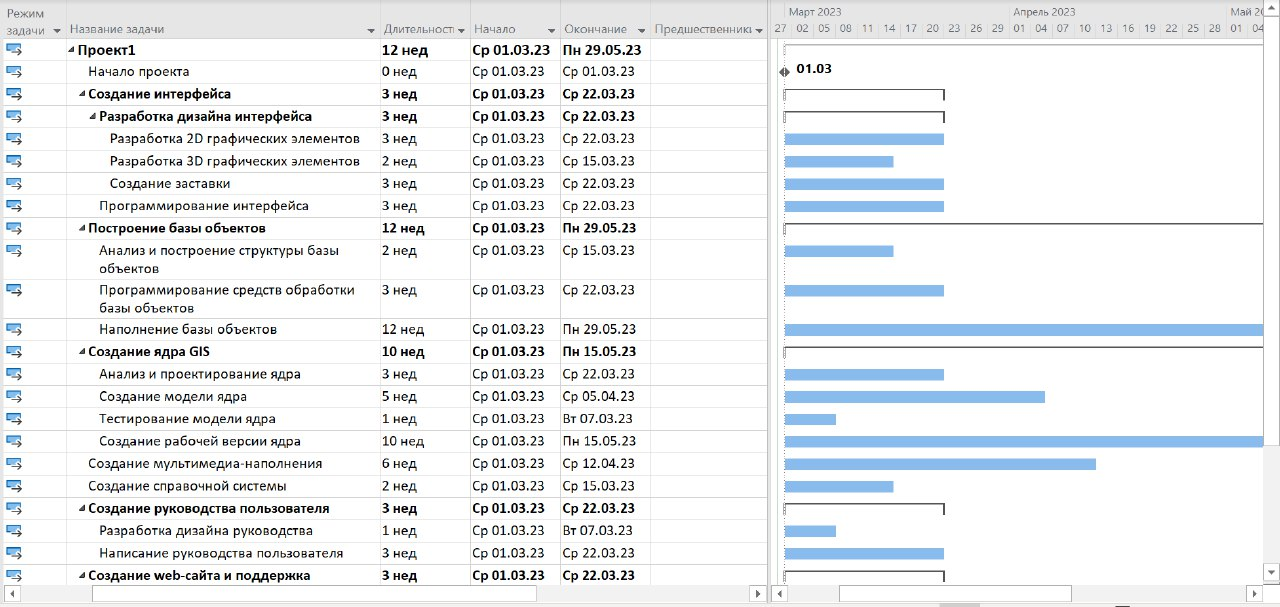
\includegraphics[scale=0.5]{inc/img/task3.jpg}
	\end{center}
	\captionsetup{justification=centering}
	\caption{Структурированный список задач}
	\label{img:task3}
\end{figure}

\section*{Задание 4}

Были установлены связи между работами. Построенная диаграмма Ганта представлена на рисунке \ref{img:task4}. Из полученного результата видно, что длительность проекта составила 27,6 недель, датой завершения работ является пятница 15.09.2023.

\begin{figure}[H]
	\begin{center}
		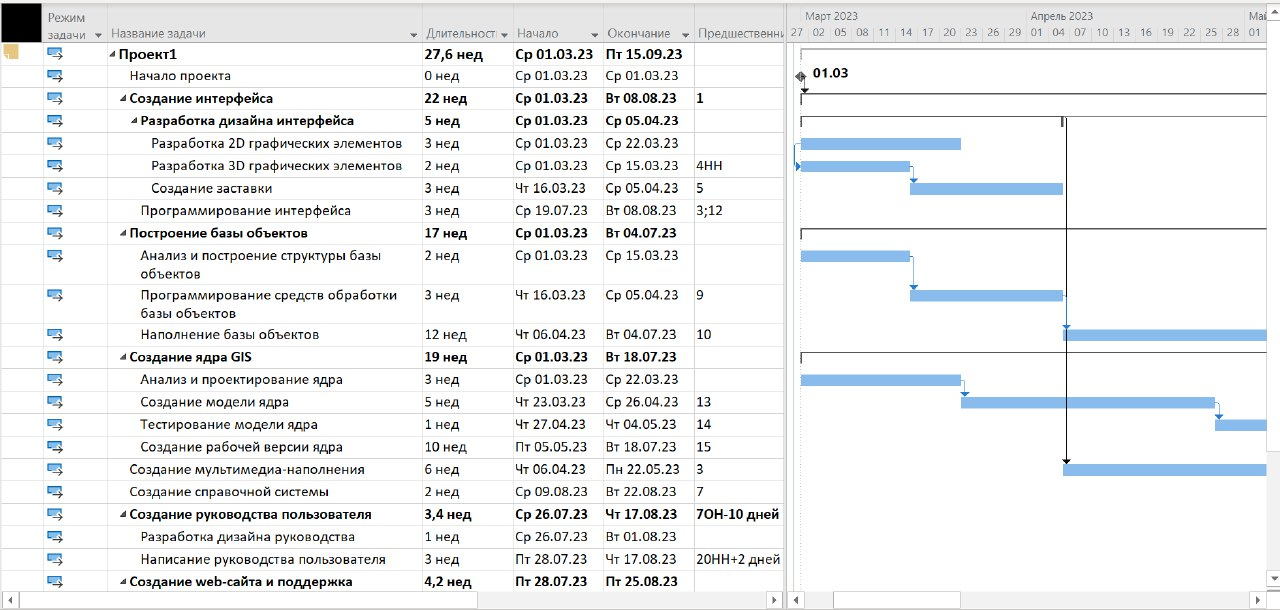
\includegraphics[scale=0.5]{inc/img/task4.jpg}
	\end{center}
	\captionsetup{justification=centering}
	\caption{Построенная диаграмма Ганта}
	\label{img:task4}
\end{figure}

\section*{Вывод}

При выполнении лабораторной работы были освоены возможности программы Microsoft Project для планирования проекта по разработке программного обеспечения.

Планирование создания карты города на основе модуля отображения в программе Microsoft Project показало, что проект не может быть завершен по истечении шести месяцев, так как его длительность превышает назначенный срок на 15 дней.
